\section{Types and validation}
\label{sec:types}
A type system and algorithm which shortly will become the main interest is the Hindley-Milner type system and the Damas-Milner Algorithm W.
The Hindley-Milner type system are the natural semantics which the Damas-Milner Algoritm W (or any other inference algorithm that infers types that the Hindley-Milner type system accepts) must adhere to.
The Damas-Milner Algorithm W is a child of an observation, that one can traverse the typing rules of Hindley-Milner backwards.
The Damas-Milner Algorithm W reconstructs types by first introducing types as unknowns, and then constraining these unknown types as more information is gathered by an operation named \textit{unification}.
\subsection{Notation}
In the world of type theory we use natural deduction to prove type validity.
Natural deduction is expressed by \textit{inference rules}, which consist of one or more premises and a conclusion.
For instance the modus ponens rule which states that if ``if $a$ implies $b$ and $a$, then $b$'', can easily be written in inference rules, where $a \rightarrow b$ and $a$ are the premises and $b$ is the conclusion (\autoref{fig:not:inf}).
\begin{figure}
  \begin{mdframed}
  \begin{prooftree}
    \AxiomC{$a \rightarrow b$}
    \AxiomC{$a$}
    \BinaryInfC{$b$}
  \end{prooftree}
  \end{mdframed}
  \caption{}
  \label{fig:not:inf}
\end{figure}
Conditions can also occur rules which state what conditions must be met for the rule to apply (\autoref{fig:not:notdead}).
\begin{figure}
  \begin{mdframed}
  \begin{prooftree}
    \AxiomC{$P$}
    \AxiomC{$P$ is not dead}
    \BinaryInfC{$P$ is alive}
  \end{prooftree}
  \end{mdframed}
  \caption{}
  \label{fig:not:notdead}
\end{figure}
Furthermore, hypotheses are written $\Gamma \vdash p$ which states that under the assumption of $\Gamma$ then $p$.

%\begin{lstlisting}[language=ML,caption={Head implementation},label={lst:headimpl},mathescape=true]
%$\texttt{fun head l: List a} \rightarrow \texttt{a =}$
    %$\texttt{match l}$
        %$\texttt{| Cons x \_ } \rightarrow \texttt{x;}$
        %$\texttt{| Nil} \rightarrow \texttt{?;}$
    %;
%\end{lstlisting}
%For instance, consider the implementation of the fuction with type $\texttt{List a} \rightarrow \texttt{a}$ in \autoref{lst:headimpl}.
%A total implementation of the function cannot exist.

%The type system for the $L$ language will be the Hindley-Milner type system~\cite{hindley1969principal,milner1978theory}.

\subsection{The language of types}\label{sec:simply}
The untyped lambda calculus is exactly that, untyped.
For it to become typed, we must introduce how types occur.
A very simple type system for the how typed lambda calculus can be proved must introduce a rule for each of the lambda calculus term types Var, Let, App and Abs.
Types must occur in programs to prove correctness, as such, program variables and types are the assumption for a proof of such a program's composite expressions such that the assumption for types will become a set the program variables $\{x_1 \dots x_n\}$ paired with their respective type $\Gamma = \{(x_1 : \tau_1)\}, \dots (x_n : \tau_n)\}$.
Stating ``it is assumed that a variable $x$ of type $\tau$ occurs in $\Gamma$'' is written $\Gamma, x: \tau$.

With the aforementioned knowledge, we can develop a simple set of inference rules which can be used to prove programs with types (\autoref{fig:simpletyped}).
\begin{figure}
  \begin{mdframed}
    \begin{subfigure}[b]{0.33\textwidth}
		\begin{prooftree}
			\AxiomC{$x: \tau \in \Gamma$}
			\LeftLabel{Var}
			\UnaryInfC{$\Gamma\vdash x:\tau$}
		\end{prooftree}
    \end{subfigure}
    \begin{subfigure}[b]{0.65\textwidth}
		\begin{prooftree}
			\AxiomC{$\Gamma \vdash e_1 : \tau_1 \rightarrow \tau_2$}
			\LeftLabel{App}
			\AxiomC{$\Gamma \vdash e_2 : \tau_1$}
			\BinaryInfC{$\Gamma \vdash e_1 e_2 : \tau_2$}
		\end{prooftree}
    \end{subfigure}
		\begin{prooftree}
			\AxiomC{$\Gamma, x: \tau_1 \vdash e : \tau_2$}
			\LeftLabel{Abs}
			\UnaryInfC{$\Gamma \vdash \lambda x . e : \tau_1 \rightarrow \tau_2$}
		\end{prooftree}
		\begin{prooftree}
			\AxiomC{$\Gamma \vdash e_1 : \tau_1$}
			\LeftLabel{Let}
			\AxiomC{$\Gamma ,x : \tau_1 \vdash e_2 : \tau_2$}
			\BinaryInfC{$\Gamma \vdash \texttt{let } x = e_1 \texttt{ in } e_2 : \tau_2$}
		\end{prooftree}
  \end{mdframed}
\begin{itemize}
  \item Var states that if $x$ has type $\tau$ in $\Gamma$ then it is assumed that $x$ has type $\tau$.
  \item App states that if $e_1$ can be proved to have type $\tau_1 \rightarrow \tau_2$ and $e_2$ can be proved to have type $\tau_1$, then $e_1 e_2$ must be of type $\tau_2$.
  \item Abs states that if $e$ has type $\tau_2$ under the assumption that $x$ has some type $\tau_1$, then $\lambda x.e$ must be of type $\tau_1 \rightarrow \tau_2$.
  \item Let does not yet have an important role, since let does the exact same as a combination of App and Abs.
    Once polymorphism is introduced, Let will play an important role.
    Currently Let states that if $e_1$ has type $\tau_1$, and $e_2$ has type $\tau_2$ under the assumption that $x$ has type $\tau_1$ (from the proof that $e_1: \tau_1$ since $x = e_1$) then \texttt{let $x = e_1$ in $e_2$} must have inhabit the type $\tau_2$.
\end{itemize}
  \caption{A simple set of rules for the simply typed lambda calculus}
  \label{fig:simpletyped}
\end{figure}
\begin{exmp}
  With the rules for the simply typed lambda calculus, it becomes possible to prove the types for programs.
  Let $\lambda f.\lambda x.f x$ be a program with the type $(\tau_1 \rightarrow \tau_2) \rightarrow (\tau_1 \rightarrow \tau_2)$, the proof to which is seen in \autoref{fig:exmp:simpletyped}.
  \begin{figure}[ht]
    \begin{mdframed}[style=bigbox]
      \begin{prooftree}
                \AxiomC{$f: \tau_1 \rightarrow \tau_2 \in \{(x: \tau_1), (f: \tau_1 \rightarrow \tau_2)\}$}
              \RightLabel{Var}
              \UnaryInfC{$\{(x: \tau_1), (f: \tau_1 \rightarrow \tau_2)\} \vdash f: \tau_1 \rightarrow \tau_2$}
                \AxiomC{$x: \tau_1 \in \{(x: \tau_1), (f: \tau_1 \rightarrow \tau_2)\}$}
              \RightLabel{Var}
              \UnaryInfC{$\{(x: \tau_1), (f: \tau_1 \rightarrow \tau_2)\} \vdash x: \tau_1$}
            \BinaryInfC{$\{(x: \tau_1), (f: \tau_1 \rightarrow \tau_2)\} \vdash f x: \tau_2$}
          \LeftLabel{Abs}
          \UnaryInfC{$\{(f: \tau_1 \rightarrow \tau_2)\} \vdash (\lambda x. f x): \tau_1 \rightarrow \tau_2$}
        \LeftLabel{Abs}
        \UnaryInfC{$\{\} \vdash \lambda f.(\lambda x.f x): (\tau_1 \rightarrow \tau_2) \rightarrow (\tau_1 \rightarrow \tau_2)$}
      \end{prooftree}
    \end{mdframed}
    \caption{The proof for $\lambda f. \lambda x . fx$}
    \label{fig:exmp:simpletyped}
  \end{figure}
\end{exmp}

The simply typed lambda calculus is straightforward, but is missing some ingredients that most programming language users cannot do without, namely \textit{polymorphism}.
For instance, in the simply typed lambda calculus one would have to define an identity function \textbf{for each} different type that uses it.
If one were to bind an identity function to \textit{id}, say $\texttt{let } \textit{id} = \lambda x. x \texttt{ in } \dots$ with type $\tau_1 \rightarrow \tau_1$, where $\tau_1$ is not determined yet.
Clearly some $f: \tau_2 \rightarrow \tau_3$ and some $y: \tau_3$ cannot both be applied to \textit{id} since if $\tau_3 \equiv \tau_1$ and $(\tau_2 \rightarrow \tau_3) \equiv \tau_1$ then an infinite type must exist $\tau_2 \rightarrow (\tau_2 \rightarrow (\tau_2 \dots))$.
What we actually want is to say that $\tau_1$ can become \textbf{any} type $\tau_4$ if for every application, every instance of $\tau_1$ is replaced by $\tau_4$ in $\tau_1 \rightarrow \tau_1$.
As such, when applying \textit{id f} then the type of \textit{id} must become $(\tau_2 \rightarrow \tau_3) \rightarrow (\tau_2 \rightarrow \tau_3)$, but only for this application.
More generally the type for \textit{id} becomes \textit{generalized} and as such has the universally quantified type $\forall \tau_1. \tau_1 \rightarrow \tau_1$.

Generally, introducing polymorphism directly to the simply typed lambda calculus lifts the type system to one called System F.
System F in undecidable, and as such, the Hindley-Milner type system will be of interest instead, since it introduces polymorphism like System F, but in a restricted way such that it becomes decidable.

%Before delving into types, the lambda calculus defined in \autoref{sec:lc} must be augmented with the \textit{let expression} (\autoref{eq:letb}).
%\begin{align}
	%\texttt{let } x = Y \texttt{ in } E
	%\label{eq:letb}
%\end{align}
%It should be noted that the let binding can be expressed by abstraction and application (\autoref{eq:letaa}).
%\begin{align}
	%(\lambda x . E) (Y)
	%\label{eq:letaa}
%\end{align}
%The let expression has a nice property that will become apparent later when typing rules are introduced.

\subsection{Polymorphism and Hindley-Milner}
%Types are an artificial layer atop of a program just as spell checking is an artificial layer atop text.
There are two variants of types in the Hindley-Milner type system, the \textit{monotype} and the \textit{polytype}.
A monotype is either a type variable, an abstraction of two monotypes or an application of a type constructor (\autoref{eq:mono}).
\begin{align}
	mono \,\,\tau = a \,|\, \tau \rightarrow \tau \,|\, C \tau_1 \dots \tau_n
	\label{eq:mono}
\end{align}
\textit{Atoms} are terminal terms in a formula and are expressed either by type variable $a$ or $C$ with no type parameters.
The application term of the monotype is dependent on the primitive types of the programming language.
The types $\tau_1 \dots \tau_n$ are monotype parameters required to construct some type $C$.
In $L$ the set of type constructors are $\{ \texttt{Int}, \texttt{Bool} \} \cup \texttt{ADT}$.
\texttt{Int} and \texttt{Bool} are type constructors of arity 0 thus only have one instantiation and are atomic.
The set of constructors \texttt{ADT} encapsulates the set of program defined algebraic data type.
\begin{exmp}
    Let $\texttt{ADT} = \{ \texttt{List} \}$ where \texttt{List} is defined as in \autoref{lst:listinstance}.
    The \textit{type constructor} (not to be confused for constructors like \texttt{Cons} or \texttt{Nil}) for \texttt{List} has the signature $\texttt{a} \rightarrow \texttt{List a}$ stating that if supplied with some type \texttt{a} it constructs a type of \texttt{List a} (effectively containing the provided type).
    The type \texttt{List} is a type constructor with one type parameter \texttt{a}.
\end{exmp}

$\bot$ denotes falsity, in type systems a value of this type can never exist since that in itself would disprove the program.
It is common in programming languages with strong type systems to let thrown exceptions be of type $\bot$ since it adheres to every type and indicates that the program is no longer running, since no instance of $\bot$ can exist.
$\top$ denotes truth, in type systems every type is a supertype of $\top$.
$\top$ is in practice only used to model side effects, since not all side effects return useful values.
In programming languages with side effects $\bot$ and $\top$ are considerably more useful than in pure programming languages.

A polytype is a polymorphic type (\autoref{eq:poly}).
\begin{align}
	poly \,\, \sigma = \tau \,|\, \forall a . \sigma
	\label{eq:poly}
\end{align}
Polymorphic types either take the shape of a type variable or universally quantify some type, naming the quantifier $a$.
All type variables of $\sigma$, are not necessarily quantified, since the constraint imposed by the \textbf{Gen} rule of \autoref{fig:hmrules} constrains the domain that $a$ ranges over to contain only type variables that are not free in $\Gamma$.
The notion of free type variables and polymorphism will be explored further once the definition of free has been introduced.
%Many types may adhere to a polymorphic type but polymorphic types do not adhere to any type other than polymorphic types.

The type hierarchy of the Hindley-Milner type-system is shown in \autoref{fig:polytree}.
%The concept of adherence in types is commonly called \textit{subtyping}.
%Every subtype is a \textit{at least} an implementation of it's supertype.
%Subtyping does not occur in the same granularity in Hindley-Milner as in languages which support inheritance and down casting.
%Since this concept can be difficult to grasp from just text, observe \autoref{fig:polytree}.
\begin{figure}[ht]
    \centering
        \begin{tikzpicture}
            %\node[draw=none] (sigma) {$\sigma$};

            \node[draw=none] (top) {$\top$};

            \node[draw=none, below = of top] (t1) {$\tau$};
            \path [->] (top) edge node[left] {} (t1);

            \node[draw=none, below = of t1] (tv) {$a$};
            \node[draw=none, left = of tv] (arr) {$\tau_1 \rightarrow \tau_2$};
            \node[draw=none, right = of tv] (tc) {$C \tau_1 \dots \tau_n$};

            \node[draw=none, below = of tv] (bot) {$\bot$};

            %\path [->] (sigma) edge node[left] {} (top);

            \path [->] (t1) edge node[left] {} (arr);
            \path [->] (t1) edge node[left] {} (tv);
            \path [->] (t1) edge node[left] {} (tc);

            \path [->] (tv) edge node[left] {} (arr);
            \path [->] (tv) edge node[left] {} (tc);

            \path [->] (tv) edge node[left] {} (bot);
            \path [->] (arr) edge node[left] {} (bot);
            \path [->] (tc) edge node[left] {} (bot);
        \end{tikzpicture}
    \caption{The type hierarchy of Hindley-Milner.}
    \label{fig:polytree}
\end{figure}
Notice the lack of $\sigma$ in \autoref{fig:polytree} since $\sigma$ is but a mechanism to prove type systems.
%$\sigma$ is but a mechanism to prove type systems, $\sigma$ is never a specific type.
%\begin{remark}
    %\label{remark:polyimpl}
%An important implementation detail which should be noted is that of the polymorphic type.
%Polymorphic types can be regarded as being a pair of bound types and monotype.
%%Instead of keeping track of what types cannot occur, which will grow as the typing algorithm continues, keeping track of the ones that do occur in the monotype simplifies the implementation.
%This representation is convenient for the \textbf{Gen} rule.
%\end{remark}

A principal component of typing in Hindley-Milner is the \textit{environment}, the environment is nothing more than a more context aware name for the hypotheses.
The environment $\Gamma$ is now a set of pairs of program variable and polytype (\autoref{eq:env}), in contrast to a set of pairs of program variables and monotypes (\autoref{fig:exmp:simpletyped}).
Now $\vdash$ is enhanced such that it can also judge polymorphic types; $\Gamma \vdash x: \sigma$ signifies a \textit{typing judgment}, meaning that under the assumption of $\Gamma$, the variable $x$ can take the \textbf{poly}type $\sigma$.
\begin{remark}
    \label{remark:judgpoly}
    Notice that judging a type now, does not necessarily mean that the judged type is the only type that $x$ may take, it states that it is one \textit{possible} type that $x$ may take.
    The property of taking multiple possible types is what allows polymorphism.
    This is made more apparent in \autoref{exmp:letpoly} where \texttt{id} may take the type of either $\forall a . a \rightarrow a$, $\texttt{Int} \rightarrow \texttt{Int}$ or $\forall a . (a \rightarrow a) \rightarrow (a \rightarrow a)$.
\end{remark}
\begin{align}
	\Gamma \,\, = \epsilon \,|\, \Gamma, x : \sigma
	\label{eq:env}
\end{align}

Like in the untyped lambda calculus, types also have notions of free and bound type variables.
%Bound type variables are ones that explicitly have been introduced to the type system by either let or abstraction in the context of some expression.
Type variables occur bound when they occur in the environment (from being bound by either a let expression or abstraction) or when they occur quantified.
Type variables occur free when they are not introduced by a quantification and they do not occur in the environment.
\begin{align}
	 & \textit{free}(a) = \{ a \}                                                              \tag*{}\\
	 & \textit{free}(C \tau_1 \dots \tau_n ) = \bigcup_{i = 1}^n \textit{free}(\tau_i)           \tag*{}\\
     & \textit{free}(\tau_1 \rightarrow \tau_2) = \textit{free}(\tau_1) \cup \textit{free}(\tau_2)  \tag*{}        \\
	 & \textit{free}(\Gamma) = \bigcup_{x:\sigma \in \Gamma} \textit{free}(\sigma)             \tag*{}\\
   & \textit{free}(\forall a . \sigma) = \textit{free}(\sigma) \backslash \{ a \}                     \tag*{}
   %& \textit{free}(\Gamma \vdash x : \sigma) = \textit{free}(\sigma) - \textit{free}(\Gamma) \label{eq:diffeq}
\end{align}
%The last rule (\autoref{eq:diffeq}) of when type variables are free can be a bit tricky to grasp without understanding how monotypes occur in $\Gamma$.

Understanding how monotypes occur in the environment is of importance when generalizing types in practice.
Monotypes are just polytypes without any quantifier, such that they always occur free in $\Gamma$.
 %defines the free variables for some $\sigma$ under the assumption of some $\Gamma$ such that the definition states ``all free type variables in $\sigma$, that are not monotypes in $\Gamma$''.
Generalization of a monotype into a polytype should quantify variables that \textbf{only} occur free in that monotype, e.g. they must not occur free in any type in $\Gamma$, such that the generalisable variables of a monotype are $\textit{free}(\tau) \backslash \textit{free}(\Gamma)$.

If when generalizing monotypes, one quantifies all variables $\textit{free}(\tau)$ arbitrary monotypes that occur various places in a program may occur both polymorphic and monomorphic.
If such an event occurs, then values that have \textbf{any} type can occur ($\forall a.a$), which should not validate.
For instance, a value \textit{id} af type $\forall a.a$ would both be valid to use in the expression $\textit{id } 5$ and $\textit{id} + 5$, which clearly do different things.
\begin{remark}
  The type $\forall a.a$ is clearly an absurd type (called absurd in Haskell), since it allows one to bypass the type-system.
\end{remark}
%This rule is important, since the system may not arbitrarily generalize over monotypes.
%\begin{exmp}
%Consider the type for the function \texttt{fst} in \autoref{lst:fstimpl}.
%\begin{lstlisting}[language=ML,caption={First function},label={lst:fstimplbad},mathescape=true]
%fun fst a b: $\forall$A.$\forall$B.A $\rightarrow$ B $\rightarrow$ A = a;
%\end{lstlisting}
%\begin{lstlisting}[language=ML,caption={First function in lambda calculus},label={lst:fstimpl},mathescape=true]
%let fst = $\lambda$a.(let f = $\lambda$b.a in f) in fst
%\end{lstlisting}
    %The type for \texttt{fst} is $\forall A \forall B . A \rightarrow B \rightarrow A$.

    %Note that a naive typing could look like $\forall A  . A \rightarrow (\forall B . B \rightarrow A)$ but rank-2 polymorphism is not typable in Hindley-Milner.
    %An important realization is the context from where the type analysis is made.
    %If type analysis is made from within the bounded context of \texttt{f} the type of \texttt{f} becomes $\forall B . B \rightarrow A$ and the type variable $A$ is free.
%\end{exmp}
%The variables which may appear in a quantification have an important role in \autoref{eq:substitution}, since only free variables may be substituted.
%Free variables are also a core part of generalizing a type for inference algorithms (\autoref{subsec:algw}).
%When modelling polymorphic types with a technique such as \autoref{remark:polyimpl} finding the set of bound variables is trivial.
%\begin{align}
    %& \textit{bound}(\tau) = \textit{free}(\tau) - \textit{free}(\Gamma)
%\end{align}
%When generalizing a type $\tau$ all types which do not occur in $\Gamma$ must be quantified.
%\begin{exmp}
%\begin{gather}
    %\Gamma = \{ (\textit{x}, \gamma) \} \label{eq:monoeq}\\
%\begin{align}
    %\textit{bound}(\tau \rightarrow \gamma) &= \{\tau , \gamma\} - \textit{free}(\Gamma)\\
    %&= \{\tau , \gamma\} - \{ \gamma \} = \{ \tau \}\tag*{}
%\end{align}
%\end{gather}
%Clearly the only bound type variable in the context of $\tau \rightarrow \gamma$ is $\tau$ such that it may become $\forall \tau. \tau \rightarrow \gamma$ in the instance that the type represents a polymorphic let expression.
    %Note that $\texttt{x:}\gamma$ in \autoref{eq:monoeq} does not contain $\gamma$ as a quantified type since it has been introduced by an abstraction and \textbf{Abs} only introduces monomorphic types (\autoref{fig:hmrules}).
    %An interesting observation is that there can only exist one implementation of the above type system if $\tau \rightarrow \gamma$ is to be introduced by a polymorphic let expression which is displayed in \autoref{lst:theoremsforfree}~\cite{wadler1989theorems}.
%\begin{lstlisting}[language=ML,caption={Implementation of type state},label={lst:theoremsforfree},mathescape=true]
%$\lambda$x.
    %let z = ($\lambda$y.x) in
    %$\dots$
%\end{lstlisting}
%\end{exmp}

\section{Hindley-Milner}
With the now introduced primitives, the Hindley-Milner type system is but a set of rules composed by said primitives.
\begin{figure}
	\begin{mdframed}
		\begin{prooftree}
			\AxiomC{$x: \sigma \in \Gamma$}
			\LeftLabel{Var}
			\UnaryInfC{$\Gamma\vdash x:\sigma$}
		\end{prooftree}
		\begin{prooftree}
			\AxiomC{$\Gamma \vdash e_1 : \tau_1 \rightarrow \tau_2$}
			\LeftLabel{App}
			\AxiomC{$\Gamma \vdash e_2 : \tau_1$}
			\BinaryInfC{$\Gamma \vdash e_1 e_2 : \tau_2$}
		\end{prooftree}

		\begin{prooftree}
			\AxiomC{$\Gamma, x: \tau_1 \vdash e : \tau_2$}
			\LeftLabel{Abs}
			\UnaryInfC{$\Gamma \vdash \lambda x . e : \tau_1 \rightarrow \tau_2$}
		\end{prooftree}
		\begin{prooftree}
			\AxiomC{$\Gamma \vdash e_1 : \sigma$}
			\LeftLabel{Let}
			\AxiomC{$\Gamma ,x : \sigma \vdash e_2 : \tau$}
			\BinaryInfC{$\Gamma \vdash \texttt{let } x = e_1 \texttt{ in } e_2 : \tau$}
		\end{prooftree}

		\begin{prooftree}
			\AxiomC{$\Gamma \vdash e : \sigma_1$}
			\AxiomC{$\sigma_1 \sqsubseteq \sigma_2$}
			\LeftLabel{Inst}
			\BinaryInfC{$\Gamma \vdash e : \sigma_2$}
		\end{prooftree}
		\begin{prooftree}
			\AxiomC{$\Gamma \vdash e : \sigma$}
            \AxiomC{$a \notin \textit{free}(\Gamma)$}
			\LeftLabel{Gen}
			\BinaryInfC{$\Gamma \vdash e : \forall a . \sigma$}
		\end{prooftree}
	\end{mdframed}
	\caption{Hindley-Milner type rules}
	\label{fig:hmrules}
\begin{itemize}
    \item \textbf{Var} states that if some variable $x$ with type $\sigma$ exists in the environment, the type can be judged.
        In practice, when $x: \sigma$ is encountered in the expression tree it is added to the environment.
    \item \textbf{App} decides that if $e_1 : \tau_1 \rightarrow \tau_2$ and $e_2 : \tau_1$ has been judged to exist then $e_1 e_2$ implies the removal of $\tau_1$ from $\tau_1 \rightarrow \tau_2$ such that $e_1 e_2: \tau_2$.
    \item \textbf{Abs} is the typing rule of lambda abstractions.
        Under the assumption that $x : \tau_1$ exists in the environment, if there is a proof of $e$ having type $\tau_2$, then the abstraction of $x$ must take the type of $x$ to create the type of the body $e$; $\tau_1 \rightarrow \tau_2$.
    \item \textbf{Let} states that if $e_1$ can be proven to have type $\sigma$ under the environment $\Gamma$, and if $e_2$ can be proven to have the type $\tau$ under the environment $\Gamma, x: \sigma$, then \texttt{let $x = e_1$ in $e_2$} must have type $\tau$.
    %\item \textbf{Let} states that if $e_1$ has been judged to have type $\sigma$ then the let expression's identifier $x: \sigma$ must exist in the environment when deriving the type of $e_2$.
        %Observe that \textbf{Let} introduces a polymorphic type to the environment while \textbf{Abs} introduces a monomorphic one.
        %Note that by \autoref{remark:judgpoly} $x$ may be polymorphic in $e_2$.
    \item \textbf{Inst} specializes some polymorphic type (in regard to the type system implementation) to a more specific polymorphic type.
        $\sqsubseteq$ is the partial order of types where the binary relation between two types of how ``specific'' types are.
        In Hindley-Milner there are only universally quantified types and monomorphic types, thus $\sqsubseteq$ specifies a polytype to a monotype or a polytype to a polytype.
        For instance $\forall a . a \rightarrow a \sqsubseteq b \rightarrow b$ or $\forall a . a \rightarrow a \sqsubseteq \texttt{Int} \rightarrow \texttt{Int}$.
    \item \textbf{Gen} generalizes $\sigma$ over the type variable $a$, where $a$ must not occur free in $\Gamma$, that is, $a$ must not occur as a monomorphic type variable.
\end{itemize}
\end{figure}
There are six rules in the Hindley-Milner rules outlined in \autoref{fig:hmrules}.
Notice that \textbf{Let} introduces types to the environment as polymorphic, which is called \textit{let polymorphism}.
In contrast, \textbf{Abs} introduces types to the environment as monomorphic.

Additionally, rules which introduce numbers and arithmetic operations can easily be introduced by rules such as \autoref{fig:hm:extranum}.
\begin{figure}
  \begin{mdframed}
    \begin{subfigure}[b]{0.60\textwidth}
    \begin{prooftree}
      \AxiomC{$\Gamma \vdash x: \texttt{Int}$}
      \AxiomC{$\Gamma \vdash y: \texttt{Int}$}
      \LeftLabel{Bin op}
      \BinaryInfC{$\Gamma \vdash x + y: \texttt{Int}$}
    \end{prooftree}
    \end{subfigure}
    \begin{subfigure}[b]{0.38\textwidth}
    \begin{prooftree}
      \AxiomC{$n \in \mathbb{Z}$}
      \LeftLabel{Num}
      \UnaryInfC{$\Gamma \vdash n: \texttt{Int}$}
    \end{prooftree}
    \end{subfigure}
  \end{mdframed}
  \caption{}
  \label{fig:hm:extranum}
\end{figure}
Let polymorphism is exemplified in \autoref{exmp:letpoly}.

\begin{exmp} 
  \label{exmp:letpoly}
  Now that polymorphism has been introduced through the Hindley-Milner type system, an example naturally follows.
  Let \autoref{fig:hm:exmp1} be the proof that the program $\texttt{let } \textit{id } = (\lambda x.x) \texttt{ in let } \textit{id}_2 = (\textit{id } \textit{id}) \texttt{ in } \textit{id}_2 \, 0$ has type \texttt{Int}.
  \begin{figure}
    \begin{mdframed}[style=bigbox]
    \vspace*{0.48cm}
      \begin{subfigure}[b]{1\textwidth}
        \begin{prooftree}
                \AxiomC{$0 \in \mathbb{Z}$}
              \LeftLabel{Num}
              \UnaryInfC{$\{\textit{id }: (\forall \tau_1 . \tau_1 \rightarrow \tau_1), \textit{id}_2: \forall \tau_2. \tau_2 \rightarrow \tau_2\} \vdash 0: \texttt{Int}$}
        \end{prooftree}
        \caption{}
        \label{fig:exmp:letpoly:r4}
      \end{subfigure}
      \begin{subfigure}[b]{1\textwidth}
        \begin{prooftree}
                \AxiomC{$\textit{id}_2: \forall \tau_2. \tau_2 \rightarrow \tau_2 \in \{\textit{id }: (\forall \tau_1 . \tau_1 \rightarrow \tau_1), \textit{id}_2: \forall \tau_2. \tau_2 \rightarrow \tau_2\}$}
              \LeftLabel{Var}
              \UnaryInfC{$\{\textit{id }: (\forall \tau_1 . \tau_1 \rightarrow \tau_1), \textit{id}_2: \forall \tau_2. \tau_2 \rightarrow \tau_2\} \vdash \textit{id}_2: \forall \tau_2. \tau_2 \rightarrow \tau_2$}
              \AxiomC{$\forall \tau_2 . \tau_2 \rightarrow \tau_2 \sqsubseteq \texttt{Int} \rightarrow \texttt{Int}$}
            \LeftLabel{Gen}
            \BinaryInfC{$\{\textit{id }: (\forall \tau_1 . \tau_1 \rightarrow \tau_1), \textit{id}_2: \forall \tau_2. \tau_2 \rightarrow \tau_2\} \vdash \textit{id}_2\, : \texttt{Int} \rightarrow \texttt{Int}$}
        \end{prooftree}
        \caption{}
        \label{fig:exmp:letpoly:l3}
      \end{subfigure}
      \begin{subfigure}[b]{1\textwidth}
        \begin{prooftree}
            \AxiomC{\autoref{fig:exmp:letpoly:l3}}
            \AxiomC{\autoref{fig:exmp:letpoly:r4}}
          \LeftLabel{App}
          \BinaryInfC{$\{\textit{id }: (\forall \tau_1 . \tau_1 \rightarrow \tau_1), \textit{id}_2: \forall \tau_2. \tau_2 \rightarrow \tau_2\} \vdash \textit{id}_2 \, 0: \texttt{Int}$}
        \end{prooftree}
        \caption{}
        \label{fig:exmp:letpoly:r2}
      \end{subfigure}
      \begin{subfigure}[b]{1\textwidth}
        \begin{prooftree}
                \AxiomC{$\textit{id }: \forall \tau_1 . \tau_1 \rightarrow \tau_1 \in \{\textit{id }: (\forall \tau_1 . \tau_1 \rightarrow \tau_1)\}$}
              \LeftLabel{Var}
              \UnaryInfC{$\{\textit{id }: (\forall \tau_1 . \tau_1 \rightarrow \tau_1)\} \vdash \textit{id }: \forall \tau_1 . \tau_1 \rightarrow \tau_1$}
            \AxiomC{$\forall \tau_1 . \tau_1 \rightarrow \tau_1 \sqsubseteq \tau_2 \rightarrow \tau_2$}
          \LeftLabel{Gen}
          \BinaryInfC{$\{\textit{id }: (\forall \tau_1 . \tau_1 \rightarrow \tau_1)\} \vdash \textit{id } : \tau_2 \rightarrow \tau_2$}
        \end{prooftree}
        \caption{}
        \label{fig:exmp:letpoly:r3}
      \end{subfigure}
      \begin{subfigure}[b]{1\textwidth}
        \begin{prooftree}
            \AxiomC{$\textit{id }: (\forall \tau_1 . \tau_1 \rightarrow \tau_1) \in \{\textit{id }: (\forall \tau_1 . \tau_1 \rightarrow \tau_1)\}$}
            \LeftLabel{Var}
            \UnaryInfC{$\{\textit{id }: (\forall \tau_1 . \tau_1 \rightarrow \tau_1)\} \vdash \textit{id }: (\forall \tau_1 . \tau_1 \rightarrow \tau_1)$}
                  \AxiomC{$\forall \tau_1. \tau_1 \rightarrow \tau_1 \sqsubseteq (\tau_2 \rightarrow \tau_2) \rightarrow (\tau_2 \rightarrow \tau_2)$}
                \LeftLabel{Inst}
                \BinaryInfC{$\{\textit{id }: (\forall \tau_1 . \tau_1 \rightarrow \tau_1)\} \vdash \textit{id}: (\tau_2 \rightarrow \tau_2) \rightarrow (\tau_2 \rightarrow \tau_2)$}
        \end{prooftree}
        \caption{}
        \label{fig:exmp:letpoly:l2}
      \end{subfigure}
      \begin{subfigure}[b]{1\textwidth}
        \begin{prooftree}
                \AxiomC{\autoref{fig:exmp:letpoly:l2}}
                \AxiomC{\autoref{fig:exmp:letpoly:r3}}
              \LeftLabel{App}
              \BinaryInfC{$\{\textit{id }: (\forall \tau_1 . \tau_1 \rightarrow \tau_1)\} \vdash (\textit{id } \textit{id}): \tau_2 \rightarrow \tau_2$}
        \end{prooftree}
        \caption{}
        \label{fig:exmp:letpoly:l1}
      \end{subfigure}
      \begin{subfigure}[b]{1\textwidth}
        \begin{prooftree}
          \AxiomC{\autoref{fig:exmp:letpoly:l1}}
              \AxiomC{$\tau_2 \notin \textit{free}(\{\textit{id }: (\forall \tau_1 . \tau_1 \rightarrow \tau_1)\})$}
            \LeftLabel{Gen}
            \BinaryInfC{$\{\textit{id }: (\forall \tau_1 . \tau_1 \rightarrow \tau_1)\} \vdash (\textit{id } \textit{id}): \forall \tau_2. \tau_2 \rightarrow \tau_2$}
            \AxiomC{\autoref{fig:exmp:letpoly:r2}}
          \LeftLabel{Let}
          \BinaryInfC{$\{\textit{id }: (\forall \tau_1 . \tau_1 \rightarrow \tau_1)\} \vdash \texttt{let } \textit{id}_2 = (\textit{id } \textit{id}) \texttt{ in } \textit{id}_2 \, 0: \texttt{Int}$}
        \end{prooftree}
        \caption{}
        \label{fig:exmp:letpoly:r1}
      \end{subfigure}
      \begin{subfigure}[b]{1\textwidth}
        \begin{prooftree}
                  \AxiomC{$x: \tau_1 \in \{x: \tau_1\}$}
                \LeftLabel{Var}
                \UnaryInfC{$\{x: \tau_1\} \vdash x: \tau_1$}
              \LeftLabel{Abs}
              \UnaryInfC{$\{\} \vdash (\lambda x.x): \tau_1 \rightarrow \tau_1$}
              \AxiomC{$\tau_1 \notin \textit{free}(\{\})$}
            \LeftLabel{Gen}
            \BinaryInfC{$\{\} \vdash (\lambda x.x): \forall \tau_1 . \tau_1 \rightarrow \tau_1$}
            \AxiomC{\autoref{fig:exmp:letpoly:r1}}
          \LeftLabel{Let}
          \BinaryInfC{$\{\} \vdash \texttt{let } \textit{id } = (\lambda x.x) \texttt{ in let } \textit{id}_2 = (\textit{id } \textit{id}) \texttt{ in } \textit{id}_2 \, 0: \texttt{Int}$}
        \end{prooftree}
      \end{subfigure}
    \vspace*{0.48cm}
    \end{mdframed}
    \caption{}
    \label{fig:hm:exmp1}
  \end{figure}
\end{exmp}
%\begin{exmp}
%\label{exmp:letpoly}
%Throughout this example the convenient syntax $(x, z)$ is the pair of the variables $x$ and $z$ which can be implemented by algebraic data structures or a combinator.

%The identity function is a common example to illustrate type systems (\autoref{lst:idfun}).
%\begin{lstlisting}[language=ML,caption={Identity function in $L$},label={lst:idfun}]
%fun id x = x;
%id 4;
%\end{lstlisting}
%\begin{lstlisting}[language=ML,caption={Identity function in lambda calculus with let},label={lst:idfunlam},mathescape=true]
%let id = ($\lambda x . x$) in
%id 4
%\end{lstlisting}
%Stating that id has the type $\forall a.a \rightarrow a$ and $4$ has the type \texttt{Int} is \autoref{lst:idfunlam} program correct?
%By applying the Hindley-Milner rules one can prove or disprove this statement.
%A correct proof of \autoref{lst:idfun} must be \autoref{fig:typeexampleid}.

%\begin{lstlisting}[language=ML,caption={Identity function in lambda calculus by abstraction},label={lst:idfunlamabs},mathescape=true]
%($\lambda$id.id 4)($\lambda$x.x)
%\end{lstlisting}
%\autoref{lst:idfunlam} and \autoref{lst:idfunlamabs} are two equivalent programs with slightly different proofs which raises the question of why the let expression is even needed.
%If \autoref{lst:idfunlam} and \autoref{lst:idfunlamabs} were to be slightly changed such that two new programs \autoref{lst:idfunlam2} and \autoref{lst:idfunlamabs2} were to be proved, \autoref{lst:idfunlamabs2} would not be provable while \autoref{lst:idfunlam2} would.
%\begin{lstlisting}[language=ML,caption={Identity function with two applications},label={lst:idfunlam2},mathescape=true]
%let id = ($\lambda$x.x) in
%(id 4, id id)
%\end{lstlisting}
%\begin{lstlisting}[language=ML,caption={Identity function with two applications as abstraction},label={lst:idfunlamabs2},mathescape=true]
%($\lambda$id.(id 4, id id)($\lambda$x.x)
%\end{lstlisting}
%In \autoref{lst:idfunlamabs2} \texttt{id} cannot adhere to polymorphism by \textbf{Abs} in \autoref{fig:hmrules} whilst \textbf{Let} can.
%%\begin{figure}[ht]
    %%\begin{mdframed}[style=bigbox]
        %%\begin{subfigure}[b]{1\textwidth}
        %%\begin{prooftree}
                            %%\AxiomC{$x : a \in \Gamma$}
                            %%\LeftLabel{Var}
                        %%\UnaryInfC{$\Gamma \vdash x : a$}
                    %%\LeftLabel{Abs}
                %%\UnaryInfC{$\Gamma \vdash (\lambda x . x) : a \rightarrow a$}
                    %%\LeftLabel{Gen}
                    %%\AxiomC{$a \notin \textit{free}(\Gamma)$}
                %%\BinaryInfC{$\Gamma \vdash (\lambda x . x) : \forall a . a \rightarrow a$}
                %%\AxiomC{$\forall a . a \rightarrow a \sqsubseteq \texttt{Int} \rightarrow \texttt{Int}$}
            %%\LeftLabel{Inst}
            %%\BinaryInfC{$\Gamma \vdash (\lambda x . x) : \texttt{Int} \rightarrow \texttt{Int}$}
        %%\end{prooftree}
        %%\caption{}
        %%\label{fig:typewrongexampleid:1}
        %%\end{subfigure}
        %%\begin{subfigure}[b]{0.49\textwidth}
        %%\begin{prooftree}
                    %%\AxiomC{$\text{id} : \texttt{Int} \rightarrow \texttt{Int} \in \Gamma$}
                    %%\LeftLabel{Var}
                %%\UnaryInfC{$\Gamma \vdash \text{id} : \texttt{Int} \rightarrow \texttt{Int}$}
                    %%\AxiomC{$4 : \texttt{Int} \in \Gamma$}
                    %%\RightLabel{Var}
                %%\UnaryInfC{$\Gamma \vdash 4 : \texttt{Int}$}
            %%\RightLabel{App}
            %%\BinaryInfC{$\Gamma, \text{ id} : \texttt{Int} \rightarrow \texttt{Int} \vdash $ id 4 : \texttt{Int}}
        %%\end{prooftree}
        %%\caption{}
        %%\label{fig:typewrongexampleid:2}
        %%\end{subfigure}
        %%\begin{subfigure}[b]{0.49\textwidth}
        %%\begin{prooftree}
                %%\AxiomC{\ref{fig:typewrongexampleid:1}}
                %%\AxiomC{\ref{fig:typewrongexampleid:2}}
            %%\LeftLabel{Let}
            %%\BinaryInfC{$\Gamma \vdash $ \texttt{let} id = $(\lambda x . x)$ \texttt{in} id 4: \texttt{Int}}
        %%\end{prooftree}
        %%\caption{}
        %%\label{fig:typewrongexampleid:3}
        %%\end{subfigure}
    %%\end{mdframed}
    %%\caption{Incorrect identity function instantiation proof}
    %%\label{fig:typewrongexampleid}
%%\end{figure}
%\begin{figure}[ht]
    %\begin{mdframed}[style=bigbox]
        %\begin{subfigure}[b]{1\textwidth}
        %\begin{prooftree}
                            %\AxiomC{$\text{id} : \forall a . a \rightarrow a \in \Gamma$}
                            %\LeftLabel{Var}
                        %\UnaryInfC{$\Gamma \vdash \text{id} : \forall a . a \rightarrow a$}
                        %\AxiomC{$\forall a . a \rightarrow a \sqsubseteq \texttt{Int} \rightarrow \texttt{Int}$}
                    %\LeftLabel{Inst}
                    %\BinaryInfC{$\Gamma \vdash \text{id} : \texttt{Int} \rightarrow \texttt{Int}$}
                        %\AxiomC{$4 : \texttt{Int} \in \Gamma$}
                        %\RightLabel{Var}
                    %\UnaryInfC{$\Gamma \vdash 4 : \texttt{Int}$}
                %\RightLabel{App}
                %\BinaryInfC{$\Gamma, \text{ id} : \forall a . a \rightarrow a \vdash $ id 4 : \texttt{Int}}
        %\end{prooftree}
        %\caption{}
        %\label{fig:typeexampleid:2}
        %\end{subfigure}
        %\begin{subfigure}[b]{0.49\textwidth}
        %\begin{prooftree}
                                %\AxiomC{$x : a \in \Gamma$}
                                %\LeftLabel{Var}
                            %\UnaryInfC{$\Gamma \vdash x : a$}
                        %\LeftLabel{Abs}
                    %\UnaryInfC{$\Gamma \vdash (\lambda x . x) : a \rightarrow a$}
                        %\LeftLabel{Gen}
                        %\AxiomC{$a \notin \textit{free}(\Gamma)$}
                    %\BinaryInfC{$\Gamma \vdash (\lambda x . x) : \forall a . a \rightarrow a$}
        %\end{prooftree}
        %\caption{}
        %\label{fig:typeexampleid:1}
        %\end{subfigure}
        %\begin{subfigure}[b]{0.49\textwidth}
        %\begin{prooftree}
                %\AxiomC{\ref{fig:typeexampleid:1}}
                %\AxiomC{\ref{fig:typeexampleid:2}}
            %\LeftLabel{Let}
            %\BinaryInfC{$\Gamma \vdash $ \texttt{let} id = $(\lambda x . x)$ \texttt{in} id 4: \texttt{Int}}
        %\end{prooftree}
        %\caption{}
        %\label{fig:typeexampleid:3}
        %\end{subfigure}
    %\end{mdframed}
    %\caption{Identity function instantiation proof}
    %\label{fig:typeexampleid}
%\end{figure}
%\end{exmp}



\subsection{Damas-Milner Algorithm W}
\label{subsec:algw}
Typing rules are by themselves not that useful since they need all type information declared ahead of checking and one must deduct what types are necessary to complete a proof.
Luckily type inference is a well studied technique.
Type inference is the technique of automatically deriving types from minimal information, of which there exist many algorithms.
One of the most common inference algorithms that produce typings which adhere to the Hindley-Milner rules, is the Damas-Milner Algorithm W inference algorithm~\cite{damas1984type,damas1982principal}.
When the Damas-Milner Algorithm W discovers a new variable, it assumes that it is the most general type.
When the Damas-Milner Algorithm W discovers constraints on types, they are unified into a substitution such that the type is specified further.

For instance, in an abstraction such as $\lambda x.x + 1$ the algorithm will introduce $x$ as some type variable $\tau_1$.
When the algorithm discovers $x + 1$, it must constrain $\tau$ to have a type which must be the unification of $\tau$ and \texttt{Int}, since $+$ requires both arguments to be of type \texttt{Int}, such that $\tau$ must be substituted with the type \texttt{Int} written $\tau \mapsto \texttt{Int}$.

The Damas-Milner Algorithm W rules (\autoref{fig:dmrules}) introduce some new concepts such as \textit{fresh variables}, \textit{most general unifier}, and the \textit{substitution set}.
Fresh variables are introduced by picking a variable that has not been picked before from the infinite set $\tau_1, \tau_2 \dots $.
In the earlier example where $x$ had type $\tau$, $\tau$ was a fresh variable.
The substitution set is a mapping from type variables to types (\autoref{eq:substitution}), which in the earlier example had the instance $\tau \mapsto \texttt{Int}$.
\begin{align}
    S = \{ a_1 \mapsto \tau_1, a_2 \mapsto \tau_2 \dots , a_n \mapsto \tau_n \} 
    \label{eq:substitution}
\end{align}
A substitution written $S T$ where $T$ is an arbitrary component of Hindley-Milner like an environment in which all type variables are substituted (\autoref{fig:subsem}).
\begin{figure}
\begin{mdframed}
\begin{align}
    &S \Gamma = \{ (x, S \sigma) \,\,|\,\, \forall (x, \sigma) \in \Gamma \} \tag{Environment}\\
    &S \sigma  = 
        \begin{cases}
            S \tau & \text{if } \sigma \equiv \tau\\
            \{ a' \mapsto \tau_1 \,\,|\,\, (a', \tau_1) \in S \land (a, *) \notin S \} \sigma' & \text{if } \sigma \equiv \forall a . \sigma'
        \end{cases}
    \tag{Poly}\\
    &S (\tau_1 \rightarrow \tau_2) = S\tau_1 \rightarrow S\tau_2 \tag{Arrow}\\
    &S a = 
        \begin{cases}
            \tau & \text{if } (a, \tau) \in S\\
            a & 
        \end{cases}
    \tag{Typevariable}\\
    &S C \tau_1 \dots \tau_n = C S\tau_1 \dots S\tau_n \tag{Constructor}
\end{align}
\end{mdframed}
    \caption{Substitutions}
    \label{fig:subsem}
\end{figure}
Substitution sets can also be combined $S_1 \cdot S_2$ with well defined-semantics.
The combination of substitution sets is a key component for the correctness of the Damas-Milner inference algorithm.
\begin{align}
    S_1 \cdot S_2 = \{ (a \mapsto S_1\tau) \,\,|\,\, (a \mapsto \tau) \in S_2) \} \cup S_1
    \label{eq:combination}
\end{align}
\begin{remark}
By the substitution set combination operator transitive and circular substitutions cannot occur since type variables in $S_1$ will inherit all the mappings from $S_2$ by union.
Transitivity is avoided by substituting all instances of type variables values (the mapped to type variables) in $S_2$ with ones that occur in $S_1$.
The properties ensured by the combination semantics also induce the property of idempotence.
This property is enforced by the Damas-Milner Algorithm W inference rules.
\end{remark}
Unification is performed differently based on the context.
Unification is performed on monotypes, each of which can take one of three forms (\autoref{eq:mono}).
Unification in the context of the Hindley-Milner type system are outlined in \autoref{fig:mgu}.
%Note that the Var rules for most general unifier outlined in \autoref{fig:mgu} are commutative.
\begin{figure}
  \begin{mdframed}[style=bigbox]
		%\begin{prooftree}
			%\AxiomC{$S, \{ (\tau_1 \rightarrow \tau_2, \gamma_1 \rightarrow \gamma_2) \} \cup T $}
			%\LeftLabel{Arrow}
			%\UnaryInfC{$S,T \cup \{ (\tau_1, \gamma_1), (\tau_2, \gamma_2) \}$}
		%\end{prooftree}

		%\begin{prooftree}
            %\AxiomC{$\tau_1, \tau_2$}
            %\LeftLabel{Intro}
			%\UnaryInfC{$\emptyset, \{ (\tau_1, \tau_2) \}$}
		%\end{prooftree}
		%\begin{prooftree}
			%\AxiomC{$S, \{ (a, \tau_1) \} \cup T$}
			%\AxiomC{$a \equiv \tau_1$}
			%\LeftLabel{
				%Var empty
			%}
			%\BinaryInfC{$S, T $}
		%\end{prooftree}

		%\begin{prooftree}
			%\AxiomC{$S, \{ (a, \tau_1) \} \cup T $}
			%\AxiomC{$a \notin \textit{free}(\tau_1)$}
			%\LeftLabel{Var sub}
			%\BinaryInfC{$S \cup \{ a \mapsto S\tau_1 \}, \{ a \mapsto S\tau_1 \} \cup T$}
		%\end{prooftree}
    \vspace*{0.48cm}

		\begin{prooftree}
      \AxiomC{}
			\LeftLabel{Var equiv}
      \UnaryInfC{$\{\}, a = a$}
		\end{prooftree}

		\begin{prooftree}
      \AxiomC{$a \notin \textit{free}(\tau)$}
			\LeftLabel{Right}
      \UnaryInfC{$\{a \mapsto \tau\}, \tau = a$}
		\end{prooftree}

		\begin{prooftree}
      \AxiomC{$a \notin \textit{free}(\tau)$}
			\LeftLabel{Left}
      \UnaryInfC{$\{a \mapsto \tau\}, a = \tau$}
		\end{prooftree}

		\begin{prooftree}
			\AxiomC{$S_1, \tau_1 = \gamma_1$}
			\AxiomC{$S_2, S_1 \tau_2 = S_1 \gamma_2$}
			\LeftLabel{Arrow}
			\BinaryInfC{$S_2 \cdot S_1, \tau_1 \rightarrow \tau_2 = \gamma_1 \rightarrow \gamma_2$}
		\end{prooftree}

		\begin{prooftree}
      \AxiomC{$S, \tau_1 \rightarrow (\tau_2 \dots \rightarrow \tau_n) = \gamma_1 \rightarrow (\gamma_2 \dots \rightarrow \gamma_n)$}
			\AxiomC{$C_1 \equiv C_2$}
			\LeftLabel{Constructor}
			\BinaryInfC{$S, C_1 \tau_1, \tau_2 \dots , \tau_n = C_2 \gamma_1, \gamma_2 \dots , \gamma_n$}
		\end{prooftree}

    \vspace*{0.48cm}
	\end{mdframed}
	\caption{Rules for most general unification}
	\label{fig:mgu}
\end{figure}

%\begin{lemma}
	%Var sub and Var empty are commutative.
%\end{lemma}
%\begin{proof}
	%Var empty is trivially true since $\equiv$ is commutative and for any $a$ and $\tau_1$ the rule produces $\emptyset \cup T = T$.\\\\
    %The commutative property of Var sub comes from the realization that $S \cup \{ \tau_1 \mapsto S\tau_2 \}$ and $S \cup \{ \tau_2 \mapsto S\tau_1 \}$ lets Algorithm W accept on the same inputs.
    %Furthermor note that Algorithm W substitutes and combines substitution sets at every step of the expression tree such that transitive types never occur because of the combination semantics.
    %\begin{case}
        %The types $\tau_1$ and $\tau_2$ are first introduced and used in unification.
        %Either all future uses of $\tau_1$ will be mapped to $\tau_2$ by the substitution set or all future uses of $\tau_2$ will be mapped to $\tau_1$.
    %\end{case}
    %\begin{case}
        %$\tau_1$ has been assigned in an earlier unification.
        %If $\tau_2 \mapsto \tau_1$ any existing references to $\tau_1$ need not change since all expressions of type variable $\tau_2$ will be mapped by the rules defined in \autoref{fig:hmrules}.
        %If any future rules need the type variable $\tau_1$ and $\tau_1 \mapsto \tau_2$ is introduced to the substitution set, the substitution rules in \autoref{fig:hmrules} will substitute the type.
    %\end{case}
%\end{proof}
\begin{remark}
    The Damas-Milner algorithm W is the most popular inference algorithm for Hindley-Milner.
    Though it remains the most popular, it has some interesting competitors.
    One of which is that of the constraint solver approach which is also used in OCaml~\cite{heeren2002generalizing}.
    The constraint solver approach is a two phase type inference algorithm.
    In the first phase the algorithm inspects the expression tree and generates a set of constraints as it goes.
    After the set of constraints $C$ has been generated it then traverses the constraints and generates type variable substitutions.
    It is argued that error reporting is significantly easier in such an approach.
\end{remark}
\begin{figure}
	\begin{mdframed}[style=style1]
		\begin{prooftree}
			\AxiomC{$x: \sigma \in \Gamma$}
			\AxiomC{$\tau = \textit{inst}(\sigma)$}
			\LeftLabel{Var}
			\BinaryInfC{$\Gamma \vdash x:\tau , \emptyset$}
		\end{prooftree}
		\begin{prooftree}
			\AxiomC{$\tau_1 = \textit{fresh}$}
			\AxiomC{$\Gamma, x: \tau_1 \vdash e: \tau_2, S$}
			\LeftLabel{Abs}
			\BinaryInfC{$\Gamma \vdash \lambda x . e : S\tau_1 \rightarrow \tau_2, S$}
		\end{prooftree}

		\begin{center}
			App
		\end{center}
		\vspace{-0.7cm}
		\begin{prooftree}
			\AxiomC{$\Gamma \vdash e_1 : \tau_1, S_1 \,\,\,\, \tau_3 = \textit{fresh}$}
			\AxiomC{$S_1 \Gamma \vdash e_2 : \tau_2, S_2 \,\,\,\, S_3 = \textit{unify}(S_2 \tau_1, \tau_2 \rightarrow \tau_3)$}
			\BinaryInfC{$\Gamma \vdash e_1 e_2 : S_3 \tau_3, S_3 \cdot S_2 \cdot S_1$}
		\end{prooftree}

		\begin{prooftree}
			\AxiomC{$\Gamma \vdash e_1 : \tau_1, S_1$}
			\AxiomC{$S_1 \Gamma , x : S_1 \Gamma(\tau_1) \vdash e_2 : \tau_2, S_2$}
			\LeftLabel{Let}
			\BinaryInfC{$\Gamma \vdash \texttt{let } x = e_1 \texttt{ in } e_2 : \tau_2, S_2 \cdot S_1$}
		\end{prooftree}
	\end{mdframed}
	\caption{Algorithm W}
	\label{fig:dmrules}
\end{figure}
%\begin{remark}
%In the language $L$ a function \texttt{fun} translates to a let expressions while \texttt{let} translates to abstraction and application.
%\end{remark}
\subsection{Instantiation}
Another interesting addition introduced by algorithm W in \autoref{fig:dmrules} is \textit{inst}.
\textit{inst} naturally follows from the \textbf{Inst} rule in \autoref{fig:hmrules} but has a slightly different behaviour.
The \textit{inst} function does not specify types anymore but simply makes unification of polymorphic types possible.
\begin{align}
    &\textit{inst}(\sigma) = \{ \, a \mapsto \textit{fresh} \,\,|\,\, a \notin \textit{free}(\sigma) \, \}\sigma
    \label{eq:inst}
\end{align}
\textit{inst} (\autoref{eq:inst}) maps all bound type variables to fresh type variables in the polytype $\sigma$.
\textit{inst} is an important component to allow polymorphic types to remain polymorphic since no bound type variables may be substituted.
\begin{exmp}
    Performing some type analysis on \autoref{eq:polyid} yields a very rich example of why \textit{inst} is necessary.
    \begin{align}
      &\texttt{let } \textit{id } = (\lambda x.x) \texttt{ in } \label{eq:polyid}\\
      &\texttt{let } \textit{ap } = (\lambda x . \lambda f . f x) \texttt{ in } \tag*{}\\
      &\texttt{let } \textit{doubleid } = (\lambda x.id (id (x + 1))) \texttt{ in } \textit{doubleid} \tag*{}
    \end{align}
    %\newline
    %\begin{minipage}{\textwidth}
%\begin{lstlisting}[language=ML,caption={Polymorphic id},label={lst:polyid},mathescape=true]
%fun id x = x;
%fun ap x f = f x;
%fun doubleid x = id (id (x + 1));
%\end{lstlisting}
    %\end{minipage}
    After inferring \textit{id} and \textit{ap} the environment will contain id $\Gamma = \{ (\textit{id}, \forall a . a \rightarrow a), (\textit{ap}, \forall \gamma,\beta . \gamma \rightarrow (\gamma \rightarrow \beta) \rightarrow \beta)\}$.
    Typing the function \textit{doubleid} without the use of \textit{inst}; begin by looking at the introduced parameter \textit{x} and then the innermost expression \textit{id $(x + 1)$}. 
\begin{align}
    &\textit{bound}(\tau) = \textit{free}(\tau) - \textit{free}(\Gamma) = \{ \tau \} \tag{\textbf{Abs} intro \texttt{x} : $\tau$ }\\
    &\Gamma = \{ (\textit{id}, \forall a . a \rightarrow a), (\textit{ap}, \forall \gamma,\beta . \gamma \rightarrow (\gamma \rightarrow \beta) \rightarrow \beta), (\texttt{x}, \forall \tau . \tau) \}\\
    &\textit{unify}(\tau, \texttt{Int}) = \{ \tau \mapsto \texttt{Int} \}\\
    &\textit{unify}(a \rightarrow a, \texttt{Int} \rightarrow \mu) = \textit{unify}(\{ a \mapsto \texttt{Int} \}a, \{ a \mapsto \texttt{Int} \}\mu) \cdot \{ a \mapsto \texttt{Int} \}\\
    &= \{ \mu \mapsto \texttt{Int} \} \cdot \{ a \mapsto \texttt{Int} \} \tag*{}\\
    &= \{ \mu \mapsto \texttt{Int}, a \mapsto \texttt{Int} \} \tag*{}
    \label{eq:unifyres}
\end{align}
    This example might not look compromising but a minor change such that the body of \textit{doubleid} becomes \textit{id (ap (id $(x + 1)$))} yields an interesting problem.
    In the case of introducing \textit{ap} the two type instances for \textit{id} must be different (\textit{id} must be introduced with different type variables) to retain it's polymorphic properties.
    The following steps are performed when inferring this new body.
\begin{align}
    &\textit{unify}(\gamma \rightarrow (\gamma \rightarrow \beta) \rightarrow \beta, \texttt{Int} \rightarrow \delta) \tag{\texttt{ap (id (x + 1))} }\\
    & = \{ \gamma \mapsto \texttt{Int}, \delta \mapsto (\texttt{Int} \rightarrow \beta) \rightarrow \beta \} \tag*{}\\
    &\{ \gamma \mapsto \texttt{Int}, \delta \mapsto (\texttt{Int} \rightarrow \beta) \rightarrow \beta \} \cdot \{ \mu \mapsto \texttt{Int}, a \mapsto \texttt{Int} \} \tag{\textbf{App} $S_3 \cdot S_2$ }\\
    & = \{ \gamma \mapsto \texttt{Int}, \delta \mapsto (\texttt{Int} \rightarrow \beta) \rightarrow \beta, \mu \mapsto \texttt{Int}, a \mapsto \texttt{Int} \} \tag*{}\\
    &\textit{unify}(a \rightarrow a, ((\texttt{Int} \rightarrow \beta) \rightarrow \beta) \rightarrow \theta) \tag{\texttt{id (ap (id (x + 1)))} }\\
    &= \textit{unify}(
     \{ a \mapsto  (\texttt{Int} \rightarrow \beta) \rightarrow \beta \} a,
     \{ a \mapsto  (\texttt{Int} \rightarrow \beta) \rightarrow \beta\} \theta
    ) \cdot \{ a \mapsto  (\texttt{Int} \rightarrow \beta) \rightarrow \beta\} \tag*{}\\
    &= \{ a \mapsto (\texttt{Int} \rightarrow \beta) \rightarrow \beta, \theta \mapsto (\texttt{Int} \rightarrow \beta) \rightarrow \beta \} \cdot \{ a \mapsto (\texttt{Int} \rightarrow \beta) \rightarrow \beta\} \tag*{}\\
    &= \{ a \mapsto (\texttt{Int} \rightarrow \beta) \rightarrow \beta, \theta \mapsto (\texttt{Int} \rightarrow \beta) \rightarrow \beta \} \tag*{}\\
    &\{ a \mapsto (\texttt{Int} \rightarrow \beta) \rightarrow \beta, \theta \mapsto (\texttt{Int} \rightarrow \beta) \rightarrow \beta \} \cdot \tag{\textbf{App} $S_3 \cdot S_2$ }\\
    &\{ \gamma \mapsto \texttt{Int}, \delta \mapsto (\texttt{Int} \rightarrow \beta) \rightarrow \beta, \mu \mapsto \texttt{Int}, a \mapsto \texttt{Int} \} \tag*{}
\end{align}
    Clearly $a$ cannot map to two types which cannot be unified which is a violation of the type system.
    The apparent problem is that \textit{id} is specialized within the whole of \textit{doubleid}.
    By instantiating quantified types when they are needed cases such as this can be avoided.
    \begin{align}
        &\textit{unify}(\textit{inst}(\forall a . a \rightarrow a), \textit{inst}(\forall \tau . \tau \rightarrow \mu))\\
        & = \textit{unify}(\gamma \rightarrow \gamma, \varphi \rightarrow \mu) \tag*{}\\
        & = \{ \varphi \mapsto \mu, \gamma \mapsto \mu \} \tag*{}
    \end{align}
\end{exmp}
\subsection{Recursion}
Recursion is a trivial matter once the primitives of the Hindley-Milner type system have been introduced.
Recall that in \autoref{sec:lamrec} recursion (along with mutual recursion) was shown to be implementable by introducing functions to their own scope, the same is true for types.
Allowing recursive functions in Hindley-Milner type inference systems is a matter of letting the function be present in the environment when inferring the function's own body.
Note, however, that the type must be introduced monomorphically, or else one introduces polymorphic recursion which is undecidable.
\begin{exmp}
If the function \texttt{f} defined in \autoref{eq:recplus1} were to be typed it would need to be introduced as an unknown type to the environment before typing the body of \texttt{f}.
\begin{align}
  \texttt{let } f = (\lambda x. (f x) + 1) \label{eq:recplus1}
\end{align}
Let $\Gamma = \{ \texttt{f} : \tau, \texttt{x} :  \mu \}$.
From the application \texttt{f x} the unification \texttt{unify}$(\tau, \mu \rightarrow \gamma) = \{ \tau \mapsto \mu \rightarrow \gamma \}$ must be performed, and the resulting type for the expression is $\gamma$.
The addition operation forces \texttt{unify}$(\texttt{Int}, \gamma) = \{ \gamma \mapsto \texttt{Int} \}$.
Finally the application of the addition function $+: \texttt{Int} \rightarrow \texttt{Int} \rightarrow \texttt{Int}$ and the two expressions \texttt{f x} and $1$ such that the resulting expression type is \texttt{Int}.

\end{exmp}

\subsection{Additional language features}
In addition to the rules in \autoref{fig:dmrules} many other ergonomic features can easily be modelled once the framework has been understood.
One of the most crucial features of languages are that of decision.
\begin{lstlisting}[language=ML,caption={ADT implementation of decision},label={lst:adtdecision},mathescape=true]
type Boolean = 
    | BFalse
    | BTrue
;
fun main =
  let b = BFalse;
  fun double x = x + x;
  b (0) (double 10);
\end{lstlisting}
Decision can be implemented in a variety of ways such as in \autoref{lst:adtdecision} by the use of algebraic data type aligning very much with Church Booleans~\cite{church1985calculi}.
\begin{figure}[ht]
	\begin{mdframed}[style=bigbox]
        \begin{subfigure}[b]{1\textwidth}
            \begin{prooftree}
                \AxiomC{$\Gamma \vdash e_2 : \tau_2, S_2 \,\,\, \tau_4 = \textit{fresh} \,\,\, \Gamma, S_4 = \textit{mgu}(S_1'\cdot S_2 \cdot S_3 \tau_2, \tau_4)$}
            \end{prooftree}
            \caption{}
            \label{subfig:pt1}
        \end{subfigure}
        \begin{subfigure}[b]{0.33\textwidth}
            \begin{prooftree}
                \AxiomC{$\Gamma \vdash e_1 : \tau_1, S_1 \,\, S_1' = \textit{mgu}(\texttt{Bool}, \tau_1)$}
            \end{prooftree}
            \caption{}
            \label{subfig:pt0}
        \end{subfigure}
        \begin{subfigure}[b]{0.66\textwidth}
            \begin{prooftree}
                \AxiomC{$\Gamma \vdash e_3 : \tau_3, S_3 \,\,\, \Gamma, S_5 = \textit{mgu}(S_4 \cdot S_1'\cdot S_2 \cdot S_3 \tau_3, S_4 \tau_4)$}
            \end{prooftree}
            \caption{}
            \label{subfig:pt2}
        \end{subfigure}
        \begin{prooftree}
                \AxiomC{\ref{subfig:pt0}}
                    \AxiomC{\ref{subfig:pt1}}
                    \AxiomC{\ref{subfig:pt2}}
                \BinaryInfC{$\Gamma, S_6 \,\,\, S_6 = S_5 \cdot S_4 \cdot S_1'\cdot S_2 \cdot S_3$}
            \BinaryInfC{$\Gamma \vdash \texttt{if } e_1 \texttt{ then } e_2 \texttt{ else } e_3: S_6\tau_4, S_6$}
        \end{prooftree}
	\end{mdframed}
	\caption{Decision}
	\label{fig:decision}
\end{figure}
Rather decision can be implemented by more conventional methods than combinator logic by introducing more inference rules as in \autoref{fig:decision}.
Additional language syntax features can in most cases be implemented as decision can.
\subsection{Algebraic data types and type constructors}
To implement rules for algebraic data type one must first decide on what the type of an algebraic data type is.
If algebraic data types were implemented as in \autoref{sec:adt} the type of an algebraic data type like Boolean in \autoref{lst:adtdecision} would be \texttt{a -> a -> a} since \texttt{BFalse} and \texttt{BTrue} must have a handler each.
Implementing algebraic data type by this method does not introduce anything to the inference algorithm since every algebraic data type becomes a function.
It is common to introduce algebraic data type along type constructors, since such an implementation yields descriptive errors in comparison to generated function types.

Before delving into what type constructors and algebraic data types are, we must understand what a \textit{sum-type} and a \textit{product-type} is.
Product-types are in simply terms n-arity tuples expressed by the conjunction operator $\times$ such that a two-arity tuple of type \texttt{Int} becomes \texttt{Int $\times$ Int}.
Sum-types are in informal terms a unifying umbrella, in which product-types can have a unified name.
Sum-types lets us reason with product types of different shapes, as if they were the same type.
A sum-type which we have seen earlier is the \texttt{Boolean} sum-type that can take the value of the product-type \texttt{BFalse} and \texttt{BTrue}.
The sum-type \texttt{Boolean} combines two nullary (nullary becomes the singleton $1$ in type theory) product-types by the disjunction operator $+$ \texttt{1 + 1}.
More exotic types, such as \texttt{List}, also requires \textit{type-constructor}s to become generalized.
A type constructor in type theory is denoted as abstraction in lambda calculus, such that \texttt{List a} becomes $\lambda a$ (note this is not the full type for \texttt{List}, that comes later).
Recursion in type theory is denoted by the special abstraction operator $\mu$.
Now we have all ingredient to represent a type such as \texttt{List a}; $\lambda a.\mu \textit{rec}.1 + (a \times \textit{rec})$.

%On the value level of this implementation, sum-types exist only at the level of types.

%Fortunately type constructors are present in Hindley-Milner such that it becomes a matter of implementing \texttt{sum-types}, that is, algebraic data types.

Now it only becomes a matter of introducing sum-types and product-types to the system.
Sum-types will exist purely on the type level and product-types will exist purely on the value level.


The \texttt{List} algebraic data type has the constructor \texttt{Cons} which requires a value of type \texttt{a} and a value of type \texttt{List a}.
To infer \texttt{Cons}, we must acquire a fresh variable $\gamma$ for each type constructor parameter of \texttt{List}, that is, \texttt{a} such that the type becomes \texttt{List} $\gamma$.
Now all instances of \texttt{a} in the constructor declaration of \texttt{Cons} must be substituted by $\gamma$, such that \texttt{Cons $\gamma$ (List $\gamma$)}.

In the case of construction, the product type \texttt{Cons $\gamma$ (List $\gamma$)} must be unified with the inferred type of the constructor.
When the subsequent \texttt{List} sum-type appears in the constructor, the appropriate case is handled by substituting the type parameters in the product type declaration like above.

In the case of matching, the program variables are introduced into $\Gamma$, such that for a case of \texttt{Cons x xs} the types are introduced monomorphically into $\Gamma$ as $\Gamma,x:\gamma,xs:(\texttt{List } \gamma)$.

%Fortunately type constructors are trivial to model in Hindley-Milner since a type constructor is a type lambda and rank-1 type lambdas are simply quantified types.
%Type con
%\autoref{lst:listadt} introduces the type constructor \texttt{a $\rightarrow$ List a} with value constructors \texttt{Cons: $\forall$a.a $\rightarrow$ List a $\rightarrow$ List a} and \texttt{Nil: $\forall$a.List a}.
%For instance let some program be \texttt{Cons 1 (Cons 2 Nil)} such that inference becomes a matter of first unifying the type of \texttt{Cons} and \texttt{$\forall$a.Int $\rightarrow$ List a $\rightarrow \tau_1$} using the application rule and then unifying \texttt{$\forall$a.Int $\rightarrow \tau_1 \rightarrow \tau_2$} with \texttt{Cons} again by application.


\section{The cost of expressiveness}
Modern languages with strong type systems tend to be notoriously slow to type on pathological inputs.
In fact, many languages with strong type systems provide type systems expressive enough to be Turing-complete.

In the construction of the compiler for $L$, one target was the C++ language.
An instance of a pathological input for the C++ type checker is most definitely the untyped lambda calculus.
The lambda terms in C++ must adhere to polymorphism in many cases which leads to some unknown but large blowup in compilation time.
In fact type polymorphism is commonly the root of blowup in typing.

ML, which implements a Hindley-Milner inference system, was believed to have linear complexity before shown to be exponential along with other problematic complexity findings~\cite{mairson1989deciding}.
As it will turn out, Hindley-Milner also suffers an explosive worst case induced by a pathological input fueled by polymorphism.

\begin{lemma}
    There exists a family of programs which are typeable in Hindley-Milner and produce $\Omega(2^n)$ unique type variables.
\end{lemma}
\begin{proof}
    The basis of the blowup stems from the introduced fresh type variables in the polymorphic \texttt{Let} inference rule.
    If the number of type variables can be shown to be exponential, the running time must be at least the same by operations, such as subsection set combination and unification.
    \begin{align}
      &\texttt{let } \textit{dup } = (\lambda a .\lambda f . f a a) \texttt{ in } \label{eq:ppe}\\
      &\texttt{let } \textit{deep } = (\lambda x . \textit{dup } (\textit{dup } (\textit{dup } (\dots)))) \texttt{ in } \dots \tag*{}\\
    \end{align}
%\begin{minipage}{\textwidth}
%\begin{lstlisting}[language=ML,caption={Nested dup},label={lst:pairproof},mathescape=true]
%fun dup a f = f a a;
%fun deep x = dup (dup (dup ($\dots$ x)));
%\end{lstlisting}
%\end{minipage}
    \autoref{eq:ppe} builds a large function signature for \textit{deep}.
    The innermost \textit{dup} invocation will have its signature unified to $x \rightarrow (x \rightarrow x \rightarrow \tau) \rightarrow \tau$, if \texttt{a} has type $x$ and \texttt{f} has type $x \rightarrow x \rightarrow \tau$ for some unknown $\tau$ by the App rule in \autoref{fig:dmrules}.
    The second innermost \textit{dup} invocation has the signature $((x \rightarrow x \rightarrow \tau) \rightarrow \tau) \rightarrow (((x \rightarrow x \rightarrow \tau) \rightarrow \tau) \rightarrow \gamma) \rightarrow \gamma$.
    Naively one might judge \autoref{eq:ppe} to run in $\Omega(2^n)$ but an important observation for why \autoref{eq:ppe} does not induce exponential blowup is the uniqueness of the type variables.
    If an efficient representation of \textit{dup} was implemented such that the left and right side were shared such that $\mu \mapsto ((x \rightarrow x \rightarrow \tau) \rightarrow \tau)$, the number introduced type variables would be $O(n)$.
    \begin{align}
      &\texttt{let } \textit{tuple } = (\lambda a . \lambda b . \lambda f . f a b) \texttt{ in } \label{eq:ppexp}\\
      &\texttt{let } \textit{one } = \textit{tuple } \textit{tuple } \textit{tuple } \texttt{ in } \tag*{}\\
      &\texttt{let } \textit{two } = \textit{tuple } \textit{one } \textit{one } \texttt{ in } \tag*{}\\
      &\texttt{let } \textit{three } = \textit{tuple } \textit{two } \textit{two } \texttt{ in } \tag*{}
    \end{align}
%\begin{lstlisting}[language=ML,caption={Nested tuples with different type variables},label={lst:pairproofexp},mathescape=true]
%fun tuple a b f = f a b;
%fun one = tuple tuple tuple;
%fun two = tuple one one;
%fun three = tuple two two;
%$\dots$
%\end{lstlisting}
    The trick to induce an exponential running time is demonstrated with the pathological program in \autoref{eq:ppexp}.
    By allowing \textit{tuple} to be polymorphic and have having two polymorphic parameters, every time \textit{tuple} is instantiated, it will contain only fresh variables.
    The type of \textit{tuple} is $a \rightarrow b \rightarrow (a \rightarrow b \rightarrow c) \rightarrow c$.
    Clearly this looks very much like \autoref{eq:ppexp}, but has the subtle difference of letting the parameters \textit{a} and \textit{b} (within the type instantiation of the let expression \textit{tuple}) be polymorphic and introducing every ''step`` as a polymorphic let expression.
    The return type of \textit{one} (the type of \textit{f}) is displayed in \autoref{eq:instexp}.
    \begin{align}
        \textit{inst}(a \rightarrow b \rightarrow (a \rightarrow b \rightarrow c) \rightarrow c) \rightarrow \textit{inst}(a \rightarrow b \rightarrow (a \rightarrow b \rightarrow c) \rightarrow c) \rightarrow \gamma \rightarrow \gamma.
        \label{eq:instexp}
    \end{align}
    The first and second instantiations will contain different type variable such that they are not structurally equivalent (\autoref{eq:afterinstexp}).
    \begin{align}
        (\tau \rightarrow \mu \rightarrow (\tau \rightarrow \mu \rightarrow \phi) \rightarrow \phi) \rightarrow (\varphi \rightarrow \zeta \rightarrow (\varphi \rightarrow \zeta \rightarrow \delta) \rightarrow \delta) \rightarrow \gamma \rightarrow \gamma.
        \label{eq:afterinstexp}
    \end{align}
\end{proof}
An interesting observation is that by increasing the amount of polymorphic parameters to some $c$ the number of type variables becomes $\Omega(c^n)$.
This observation does not have any significant impact since $O(f(n)) \supseteq \Omega(n^n)$ where $f$ is the algorithm for type inference, such that the problem of type inference in Hindley-Milner is at least in EXPTIME, which contains problems solvable in both $O(2^n)$ and $O(n^n)$.
The upper bound which states that type inference in Hindley-Milner is in fact \text{EXPTIME-complete} was justified in~\cite{kfoury1990ml,mairson1989deciding}.
Running the program \autoref{lst:pairproofexp} in $L$ yields a blowup of $2^n$ (\autoref{lst:appedix:bigexp}).
\autoref{fig:expplot} shows the relationship between the program typed in $L$ and the theoretical time of $2^n$.
\begin{lstlisting}[language=ML,caption={Nested tuples with different type variables},label={lst:pairproofexp},mathescape=true]
fun tuple a b f = f a b;
fun one = tuple tuple tuple;
fun two = tuple one one;
fun three = tuple two two;
fun four = tuple three three;
fun main = 0;
\end{lstlisting}
\begin{figure}[ht]
    \centering
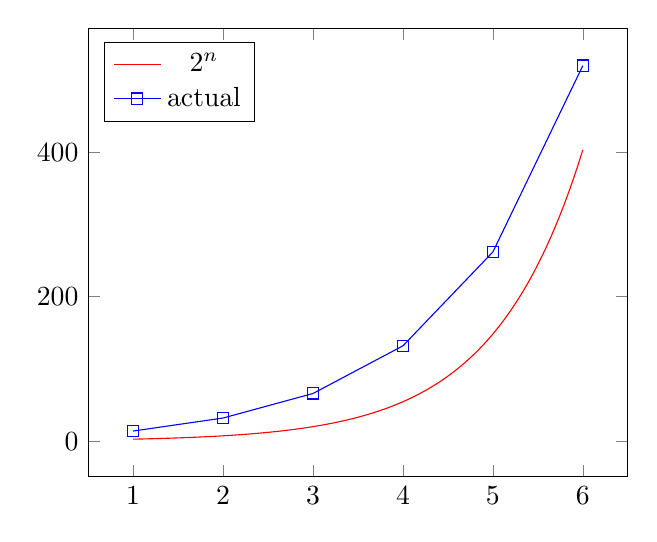
\begin{tikzpicture}
    \begin{axis}[
        legend pos= north west
        ]
       \addplot[
            domain=1:6,
            samples=100,
            color=red
        ]{exp(x)};
        \addlegendentry{$2^n$}

        \addplot[
            color=blue,
            mark=square
        ]
        coordinates {
(1,14)  (2,32)  (3,66) (4,132) (5,262) (6,520)
        };
        \addlegendentry{actual}

        %\addplot[
            %color=green,
            %mark=triangle
        %]
        %coordinates {
%(1,47)  (2,78) (3,128) (4,211) (5,347) (6,570)
        %};
        %\addlegendentry{fitted}

   \end{axis} 
\end{tikzpicture}
    \caption{Plot of type variables in Hindley-Milner type systems}
    \label{fig:expplot}
\end{figure}

\section{Higher level type systems}
The Hindley-Milner type system is a constrained variant of more general type systems.
The typed lambda caculus can come in various forms, the simplest of which is the simply typed lambda calculus (\autoref{fig:simpletyped}).
Throughout this section we have explored a type system that introduces polymorphism and type constructors.

\subsection{System F}
System F generalizes the notion of polymorphism by letting terms become polymorphic within other polymorphic types.
System F allows exotic types such as the signature $\forall a.\forall c.(\forall b.b \rightarrow \texttt{Int}) \rightarrow a \rightarrow c \rightarrow \texttt{Int}$, which could be a function that takes two potentially different typed values $a$ and $c$ and turns them into an integer and adds them (\autoref{lst:rankn}).
\begin{lstlisting}[language=ML,caption={Rank 2 type in System F},label={lst:rankn},mathescape=true]
fun f makeNum a c =
    (makeNum a) + (makeNum c);
\end{lstlisting}
We say that a type has a rank when interesting ourselves with nested quantification.
The type of by the function in \autoref{lst:rankn} requires rank-2 types to be expressible.
Generally, when quantifiers occur on the left side of $\rightarrow$ they must be locally quantified thus they increase the rank.
Unfortunately checking System F is undecidable, thus sound inference is not possible~\cite{wells1999typability}.
%System F is very powerful, since there are no constraints on how types are quantified.

\subsection{System F\underline{$\omega$}}
System F\underline{$\omega$} is orthogonal with System F, despite the similar name.
System F\underline{$\omega$} introduces type constructors, which have already been explored.
Generally, System F\underline{$\omega$} introduces a rule that allows types to become parameterized, like abstraction in the lambda calculus, such that a type that depends on a parameter $a$ may occur as $\lambda a.\tau$.
For instance, a generalized tuple may be have the type $\lambda a.\lambda b.a \times b$.
System F\underline{$\omega$} by itself is not of particular interest, since one cannot introduce generalized types without System F.

\subsection{Dependent types}
System F\underline{$\omega$} and System F are orthogonal, but compliment each other well and can represent types similar to types that can occur in traditional programming languages.
Dependent types on the other hand, introduce something quite different.
Dependent types introduce the notion of letting types be a product of an expression.
Allowing expressions to become a part of the type system, significantly increases the preciseness of types.
Dependent types are the foundation of many theorem provers, since one can encode various problems into programs.
For instance, one can precisely define the type for a matrix matrix multiplication.
Let two matrices $m_1$ with the dimensions $i$ and $j$ encoded into $m_1$'s type, and $m_2$ with the dimensions $j$ and $j$ encoded into $m_2$'s type, be multiplied, then the resulting matrix $m_3$ has the dimensions $i$ and $k$.

%The Hindley-Milner type system can only express relatively simple programs which robs algorithmic elegance in respect to other type systems.
%One domain of programs that Hindley-Milner cannot express are those that rely on \textit{rank-n types}.
%Rank-n types deals with letting abstractions have polymorphic parameters such that a type can be quantified within another type, having its depth bounded by n (rank-\textbf{n}).
%For instance \autoref{lst:rankn} is not typable in Hindley-Milner since its type is \texttt{$\forall\tau$.($\forall\gamma$.$\gamma \rightarrow$ Int) $\rightarrow \tau \rightarrow$ Int}.
%\begin{lstlisting}[language=ML,caption={Program that requires rank-n types},label={lst:rankn},mathescape=true]
%fun f makeNum a =
    %((makeNum a) + (makeNum 0)) + (makeNum (0 == 2))
%\end{lstlisting}
%More generally, any type which is quantified on the left side of $\rightarrow$ cannot be moved out thus increases the rank.

%Even languages which are typed and inferred by Hindley-Milner like Ocaml have introduced kinds through modules to allow higher-kinded types.
%Hindley-Milner is in fact a restricted version of another more general type system called \textit{System F} (and System F\underline{$\omega$}).
%The Hindley-Milner type system introduces abstractions as monomorphic types whereas System F allows any type to be polymorphic.
%It turns out that allowing higher rank polymorphism makes type inference (type reconstruction in older literature) \textit{undecidable}~\cite{wells1999typability}.
%\begin{remark}
    %Formal type systems are in their essence deductive systems, which have provable properties such as \textit{decidability}.
    %Decidability in deductive systems is a property which expresses whether a system can be decided by an algorithm (which relates to the encoding of algorithms on theoretic computers).
    %If and only if every valid formula (type) in the deductive system (type system) can have its correctness decided (and reconstructed if necessary) algorithmically.
%\end{remark}

%Another variant of type system is \textit{System F\underline{$\omega$}}.
%System F\underline{$\omega$} introduces another feature (System F\underline{$\omega$} is different to System F, it is not an extension) called type constructors.
%It is uncommon to use System F\underline{$\omega$} on its own since it only allows type constructors of monomorphic types (System F introduces polymorphism), which does not yield much expressiveness since only specific types such as \texttt{Int $\rightarrow$ List Int} would be expressible.
%Throughout this chapter, type constructors have already been introduced in such a way that they can occur in Hindley-Milner though algebraic data types such as \texttt{$\forall$a.a $\rightarrow$ List a}.
%Very commonly, moderately generalized types need both the higher rank polymorphism implied by System F and the type constructors implied by System F\underline{$\omega$}.

%Hindley-Milner can only take advantage of System F\underline{$\omega$} for rank 1 types which significantly constrains the generalization level.
%A more expressive version of Hindley-Milner is System F$\omega$ which in fact, is the basis for the type system of Haskell, which is significantly more expressive than Hindley-Milner.
%\begin{remark}
    %Haskell has introduced some additional tweaks to System F$\omega$ to avoid the decidability problem among others.
%\end{remark}

%In more expressive functional programming language type systems it has become increasingly popular abstract over implementations by introducing concepts from \textit{category theory}.
%Naturally many abstractions of category theory require rank-2 polymorphism.
%More generally the larger the level of polymorphism allowed the larger the possible abstraction level becomes.
%For instance a general purpose \textit{functor} is implementable and usable with rank-2 polymorphism while a natural transformation becomes a matter of rank-3 polymorphism.
%\begin{remark}
    %A functor is a mapping that maps from type constructor instance to another, which for instance can be a functor for lists which provides the algebra \texttt{$\forall$a.$\forall$b.List a $\rightarrow$ List b}.
%\end{remark}
%\noindent To generalize functor one must be able to express \textit{kinds} which are the types of type constructors denoted $* \rightarrow *$ for a type constructor that takes some type $*$ and creates some type $*$.
%$* \rightarrow *$ is a unary type constructor whereas $*$ is an atomic type like \texttt{Int} or \texttt{List Int}, since these types are fully applied.
%Kinds allow partial application on type constructors on a general level, since the only specific constraint is the shape and not where variables appear.
%The relaxation of type constructions allow various types to be generalized such as \texttt{a $\rightarrow$ b $\rightarrow$ M a b} which could also have the signature of \texttt{a $\rightarrow$ b $\rightarrow$ M b a} which kinds abstract over generalizing $M$ to $* \rightarrow * \rightarrow *$.
%The kind for \texttt{List} is $* \rightarrow *$ such that for any $\tau$ with kind $* \rightarrow *$ the type for functor map is \texttt{$\forall\tau$.($\forall$a.$\tau$a) $\rightarrow$ ($\forall$b.$\tau$b)}.
%\begin{remark}
    %Kinds are an abstraction which can exist purely theoretical without robbing the type system of expressiveness.
    %Just as some complications in type systems are resolved with weakening the type system or enriching the syntax, kinds can bu abstracted away into types~\cite{weirich2013system}.
%\end{remark}

%$\lambda$P introduces \textit{Dependent types} which lets types depend on terms in the language.
%A common example to show what dependent types can do is that of combining two lists $v_1$ and $v_2$ of size $n_1$ and $n_2$ into a list $v_3$ of size $n_1 + n_2$, where the size can be expressed in the type system.
%The signature for such a function in $L$ could be \texttt{$\forall a.$List $n_1$ a $\rightarrow$ List $n_2$ a $\rightarrow$ List $(n_1 + n_2)$ a}.
%Clearly one would have rules for lists such as a base case for the empty list \texttt{fun empty = Nil} with type \texttt{$\forall a.$List 0 a}, which indicates how the type system is lifted to a logical proofing tool.

\begin{figure}
    \centering
    \begin{tikzpicture}
        \matrix (m) [matrix of math nodes,
        row sep=3em, column sep=3em,
        text height=1.5ex,
        text depth=0.25ex]{
                    & \lambda\omega             &              & \lambda\Pi\omega             \\
        \lambda 2   &                           & \lambda\Pi 2                                \\
                    & \lambda\underline{\omega} &              & \lambda\Pi\underline{\omega} \\
        \lambda{\to}&                           & \lambda\Pi  \\
        };
        \path[-{Latex[length=2.5mm, width=1.5mm]}]
        (m-1-2) edge (m-1-4)
        (m-2-1) edge (m-2-3)
                edge (m-1-2)
        (m-3-2) edge (m-1-2)
                edge (m-3-4)
        (m-4-1) edge (m-2-1)
                edge (m-3-2)
                edge (m-4-3)
        (m-3-4) edge (m-1-4)
        (m-2-3) edge (m-1-4)
        (m-4-3) edge (m-3-4)
                edge (m-2-3);
    \end{tikzpicture}
    \captionsetup{singlelinecheck=off}
    \caption[nothing, items]{
        \begin{itemize}
            \item$\lambda\rightarrow$ is the simply typed lambda calculus without polymorphism.
            \item$\lambda\underline{\omega}$ is System F\underline{$\omega$}.
            \item$\lambda 2$ is System F.
            \item$\Pi$ introduces dependent types.
            \item Various combinations of the aforementioned type systems can occur as they are combined by the diagram.
              For instance, $\lambda\omega$ is System F$\omega$, the combination of $\lambda2$ and $\lambda\underline{\omega}$.
        \end{itemize}
    }
    \label{lambdacube}
\end{figure}
\autoref{lambdacube} shows the \textit{lambda cube}, introduced in \cite{barendregt1991introduction} which encapsulates the family of formal type systems.
%Complicated type system such as the \textit{calculus of constructions} ($\lambda\Pi\underline{\omega}$) are used in proof assistants since they essentially are deduction systems.
\section{Concluding remarks}
This section should act as an introduction to more general type systems and where Hindley-Milner is placed on the type system map.
Hindley-Milner by itself, is a retrofitted version of System F.
Hindley-Milner is a small part of a larger more general system which has significant impact on the extensibility of Hindley-Milner.
Some very renown functional programming languages began by implementing Hindley-Milner as their type system since it is very fast in practice and relatively simple to implement.

